\documentclass[11pt]{article}

\usepackage[a4paper,margin=1in]{geometry}
\usepackage{amsmath,amssymb,amsthm,mathtools}
\usepackage{graphicx}
\usepackage{booktabs}
\usepackage{enumitem}
\usepackage{hyperref}
\usepackage{xcolor}
\usepackage{microtype}
\setlength{\emergencystretch}{2em}

\hypersetup{colorlinks=true,linkcolor=black,citecolor=blue!50!black,urlcolor=blue!50!black}

\newtheorem{definition}{Definition}
\newtheorem{proposition}{Proposition}
\newtheorem{lemma}{Lemma}
\newtheorem{corollary}{Corollary}
\newtheorem{conjecture}{Conjecture}
\newcommand{\Arec}{\mathcal A_{\rm rec}}
\newcommand{\Astar}{\mathcal A_*}
\newcommand{\HS}{\mathrm{HS}}
\newcommand{\Tr}{\operatorname{Tr}}
\newcommand{\id}{\operatorname{id}}
\newcommand{\Ad}{\operatorname{Ad}}

\title{\textbf{Complete Record Edges, Path Holonomy, and Recovery-Correctable Readouts}\\
\large Tau Core Technical Paper II (Series Paper III)}
\author{Jozsef Olcsak\\\small Independent researcher}
\date{Draft v0.1 --- Last revised: 29 August 2026}

\begin{document}
\maketitle

\begin{abstract}
We isolate a finite technical question arising in morphological readout
frameworks: under what conditions can a source-side action separation be
identified exactly with an observer-carrier Uhlmann chord?  A reversible
\emph{complete record edge} is defined as a source-owned, trace- and
dagger-preserving relation between occupied finite record algebras, equipped
with one common action unit and no terminal bypass.  Primitive-defect
extensivity then forces an exact Trace--Gram law on the supported endpoint
pair.  Composable complete edges form a groupoid, but endpoint-only descent is
valid only when relative holonomy is null under a source-frozen operational
descriptor or belongs to a declared Uhlmann gauge.

We then separate this reversible theorem from irreversible record formation.
A three-qubit bit-flip construction gives an explicit non-isomorphic CPTP map
with an exact recovery on its occupied logical operator system.  Monotonicity
in both directions proves preservation of fidelity and hence of the Uhlmann
chord on that system.  By contrast, commuting records alone cannot distinguish
reversible transport from dephasing.  This yields a seven-part occupation
certificate that adds either a coherent off-diagonal witness or a certified
recovery test to independent action, tomography, and timing measurements.
For nonexact recovery we derive an explicit Uhlmann-chord loss bound from a
uniform trace-norm error, and hence from a full-code diamond-norm certificate.
The results are representation and identifiability theorems.  They do not
prove that a physical parent source creates or occupies complete edges, that a
laboratory carrier realizes the proposed common-action law, or that Tau Core
is empirically validated.
An upstream cyclic-support theorem can select the complete source packet inside
the declared source-irredundant MVP class, but it does not by itself prove
invertible edge transport, exact recovery, or finite action--chord identity.
This is the third stage of a seven-stage foundation programme: Paper I fixes
the architecture, Paper II isolates finite source sufficiency, the present
paper asks what survives record transport, Paper IV isolates parent-law
realization, Paper V develops temporal descent and Paper VI the quantum
terminal.  Paper VII is issued as the focused VII-A--VII-C triptych.  The
regular local clock factorization and GR proper-time limit are conditionally
closed downstream of the record map; they neither strengthen exact recovery
here nor prove physical edge occupation.
In the common morphology-conditioned architecture, the record map is the
finite resolution/acceptance stage after observer access and typed terminal
precursors; recovery tests whether distinctions lost there remain correctable
on the declared occupied support.
\end{abstract}

\begin{center}
\fbox{\begin{minipage}{.90\linewidth}\small
\textbf{Upstream quotient boundary.}
Record transport begins only after the complete source characteristic
$\mathfrak c_{B,s}=(q_B,\beta_B)$ has retained every physical base modulus.
The true redundancy sector is $\ker D\mathfrak c_{B,s}$, not the full
fixed-seed fiber of $q_B$. Complete edges and recovery maps therefore act on
the occupied physical quotient and cannot be used to erase a base stiffness,
calibration or constitutive modulus hidden by the seed-only decoder.
\end{minipage}}
\end{center}

\begin{center}
\fbox{\begin{minipage}{.90\linewidth}
\textbf{Dependency and ownership box.}

\textbf{Inputs from earlier papers:} Paper I supplies the common
morphology-conditioned readout architecture and finite action variable;
Technical Paper I (series Paper II) supplies a frozen typed source signature
and occupied support. Their unrestricted physical realization and occupation
remain open.

\textbf{Results owned here:} sufficient complete-edge conditions for finite
Trace--Gram transport; descriptor-frozen path holonomy; exact and approximate
recovery statements for irreversible CP maps; the recovery-correctable toy
model; and the FOC-7 operational certificate. This paper does not infer its
source support from transport success.  The downstream scalar-15/type-II
ownership and functional-RG closure are imported only as branch status; an RG
regulator is an analysis scheme and is not a complete record edge or an
observer quantizer in the sense defined here.
\end{minipage}}
\end{center}

\begin{center}
\fbox{\begin{minipage}{0.92\linewidth}\small
\textbf{Atemporal parent-realization terminology.}
Because the Tau parent is atemporal, phrases such as \emph{Nature selects} do
not denote an external agent or a later choice. Their precise meaning is the
internal physical implication
\[
 (B_\tau^{\rm phys},s_U,\mathcal L_{\rm parent})
 \Longrightarrow \mathfrak P,
\]
together with occupation of the support of the resulting packet
$\mathfrak P$. A theorem inside a declared completion proves only
class-relative realization. It does not prove this unrestricted base--seed
arrow, and agreement of finitely many terminal readouts cannot by itself
establish ambient-source exhaustivity. Current-facing statements therefore
use \emph{parent-law realization} and \emph{physical occupation}; any retained
legacy selection language is shorthand for this same distinction.
\end{minipage}}
\end{center}

\tableofcontents
\clearpage

\section{Question and claim boundary}

\paragraph{Inherited observer co-descent convention.}
The index $O$ labels a body-side carrier candidate before operational
closure.  A regular local rank-four descent, stable observer--source quantizer
and nonzero record/effect jointly produce the operational observer and its
accessible four-dimensional world as co-readouts.  A chart or carrier alone
is insufficient.  Complete edges and recovery maps studied here transport
records inside that inherited architecture; they neither create the body nor
constitute an independent channel layer.

The record algebra also does not create the differentiable carrier on which
its records are later read.  A possible post-body representation may contain
an observer-independent derivation family $\mathfrak d_\tau$, an
observer--source restriction $R^{\mathfrak d}_{OS}$ and the visible map
$\Phi_{OS,x}=\widetilde\Phi_{OS,x}\circ R^{\mathfrak d}_{OS}$.  Complete
edges can transport records once such a packet is supplied, but their
existence does not force constant visible rank four, integrability, a
Lorentz-conformal realization, or agreement with the ROOT/M4TR carrier.
Those are upstream geometry gates, and endpoint recovery may not be used to
select them backward.

Paper II's joint-source compression is also inherited: the mixed relation
ideal, separator multiplicity/gluing data and faithful block occupation are
joint descendants of one coherent representation/state datum
$\mathfrak J_*=(\Pi_*,\varphi_*)$.  A complete edge acts only after that datum
has supplied its occupied record support.  Transport or recovery success
cannot determine $\mathfrak J_*$ backward, and therefore cannot close its
unrestricted parent-law realization or global terminal-completeness boundary.

\paragraph{Inherited minimal formation basis.}
The body entering this paper is already a stable selected nonneutral response
of one protected source-indexed law.  Its base is the physically anchored
zero-source response structure and its universal seed is a response-distinct
base-relative source class.  Without the zero-source anchor, base and seed
remain refactorization-nonidentifiable.  Complete edges and recovery success
cannot supply that missing upstream anchor or infer seed occupation backward.

Nor does record transport turn the atemporal Parent into a history store.
Stable early and later records can refine an observer's compatible class by
intersecting simultaneous Parent preimages, while leaving every already
realized early record invariant.  This history refinement does not establish
literal temporal traversal.  Record invariance alone is also weaker than
no-signalling: a common pre-choice preparation and normalized later-local
instrument are additionally required to preserve the earlier marginal.  The
full derivation belongs to Paper VI; Paper III records only the transport
boundary needed to prevent recovery from being read as past rewriting.

Let a stabilized source/body construction assign a dimensionless finite
action separation
\begin{equation}
 x_A={\mathcal X_s\over\Astar},
 \label{eq:action-separation}
\end{equation}
while an observer carrier assigns density operators \(\rho_u,\rho_v\) and the
minimum-lift Uhlmann chord
\begin{equation}
 x_Q=d_{U,\mathrm{chord}}^2(\rho_u,\rho_v)
 =\min_U\lVert W_v-W_uU\rVert_{\HS}^2
 =2\bigl(1-\sqrt{F(\rho_u,\rho_v)}\bigr).
 \label{eq:quantum-separation}
\end{equation}
The target identity is \(x_A=x_Q\).  Equality of infinitesimal Hessians is not
enough: a finite response can have the same tangent metric but differ by
nonlinear terms.  This paper therefore asks which \emph{finite source
relations} are sufficient for the identity, and how this statement changes
for irreversible completely positive (CP) maps.

The status is deliberately narrow:
\begin{itemize}
 \item complete-edge existence is an assumption about an occupied source
 relation, not a theorem that the unrestricted physical parent law realizes
 it;
 \item the Trace--Gram result is exact only on the declared occupied support;
 \item descriptor-null holonomy is operational and claim-relative, not an
 ontological erasure rule;
 \item the CP example is a recovery-correctable toy model, not an identified
 physical Tau carrier;
 \item no numerical constant, Standard-Model spectrum, or empirical anomaly is
 derived here.
\end{itemize}

\begin{figure}[t]
 \centering
 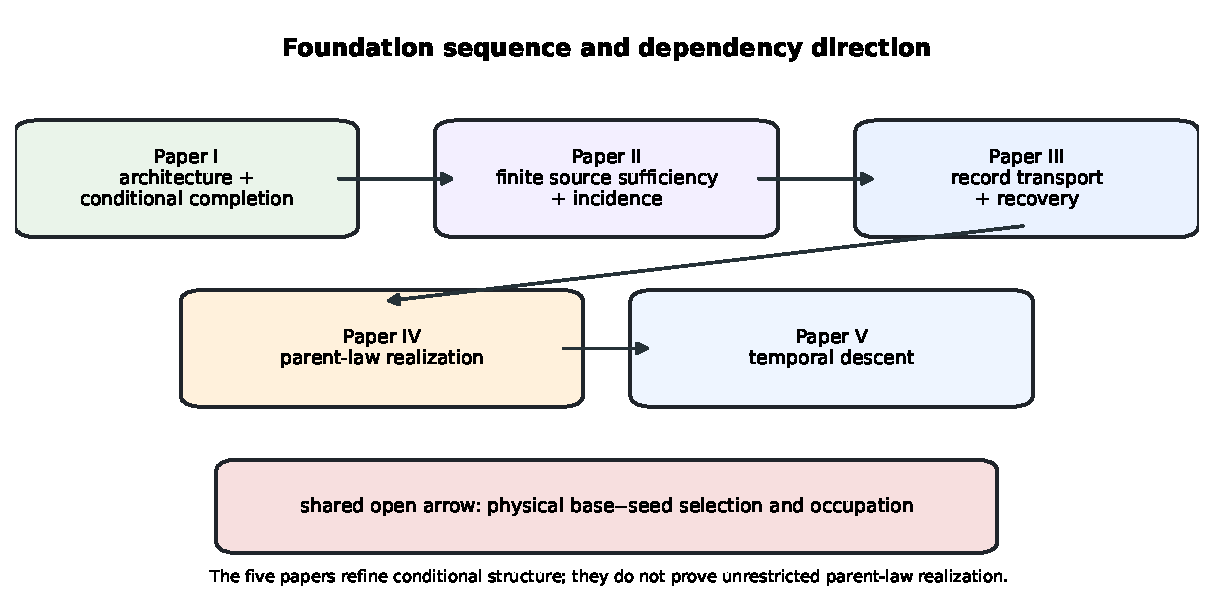
\includegraphics[width=0.92\linewidth]{figures/fig_foundation_series_map.pdf}
 \caption{Dependency direction of the foundation sequence.  Paper III starts
 from a frozen occupied source support; recovery or chord preservation cannot
 be used to infer that the physical parent selected it.}
 \label{fig:foundation-series-map}
\end{figure}

\paragraph{Series notation ledger.}
\begin{center}\small
\begin{tabular}{p{.16\linewidth}p{.53\linewidth}p{.20\linewidth}}
\toprule
Symbol & Series-wide meaning & Primary treatment\\
\midrule
\(s\) & source/seed packet prior to observer descent & Paper I\\
\(M_\tau\) & stabilized morphological body & Paper I\\
\(\operatorname{Desc}_O\) & observer-indexed physical descent/readout & Paper I\\
\(\Pi_{\rm phys}\) & selected coherent source representation & Paper II\\
\(x_A\) & normalized finite source/body action separation & Papers I, III\\
\(x_Q\) & observer-carrier Uhlmann chord separation & Papers I, III\\
\(\mathcal C,\mathcal R\) & record map and recovery map & Paper III\\
\bottomrule
\end{tabular}
\end{center}

\begin{figure}[t]
 \centering
 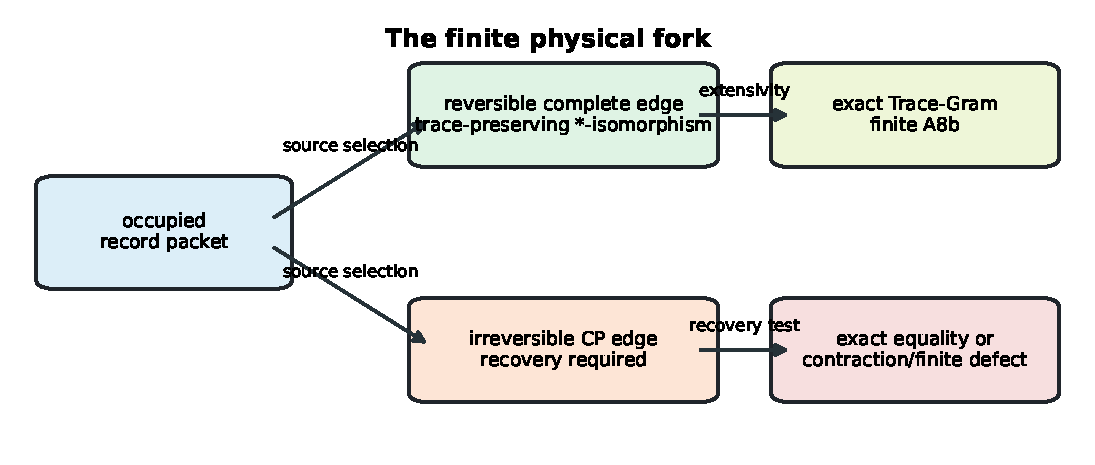
\includegraphics[width=0.93\linewidth]{figures/fig_edge_branch.pdf}
 \caption{The finite physical fork.  Exact Trace--Gram transport follows on a
 reversible complete edge.  An irreversible CP relation requires a recovery
 theorem; otherwise contraction or an additional finite defect remains.}
 \label{fig:finite-fork}
\end{figure}

\section{Finite record packet}

Let the occupied record support decompose into finitely many central blocks,
\begin{equation}
 \mathcal A_Q=\bigoplus_{\alpha=1}^m M_{n_\alpha}(\mathbb C),
 \qquad
 \tau(a)=\sum_\alpha p_\alpha\,{\Tr(a_\alpha)\over n_\alpha},
 \quad p_\alpha>0,
 \quad \sum_\alpha p_\alpha=1.
 \label{eq:finite-record-algebra}
\end{equation}
We assume a finite special dagger-Frobenius packet
\((\mathcal A_Q,\mu,\eta,\Delta=\mu^\dagger,\epsilon=\eta^\dagger)\) with
\begin{equation}
 \mu\Delta=I_{\mathcal A_Q}.
 \label{eq:specialness}
\end{equation}
Specialness makes the primitive copy map isometric in the inherited trace
metric.  It is a strong normalization condition; a merely normalizable
Frobenius algebra has \(\mu\Delta=L\) for a positive central loop operator
\(L\), leaving a possible block-dependent scale.

\begin{definition}[Finite recovery completeness]
A source law is \emph{finite recovery-complete} on an occupied family when
its finite action separation depends only on the source-owned minimum-lift
chord,
\begin{equation}
 x_A=F(x_Q),\qquad F(0)=0,
 \label{eq:finite-recovery-completeness}
\end{equation}
and no additional positive stiffness remains on the declared source support
while being invisible to that lift.  This is a sufficient-statistic
assumption for finite action separation, not a consequence of a positive
local Hessian alone.
\end{definition}

The admissible domain for exact extensivity is
\begin{equation}
 \mathcal D_2=\{(Y_1,Y_2):Y_i\geq0,\;Y_1+Y_2\leq2,\;
 Y_1,Y_2\text{ arise from admitted orthogonal source slots}\}.
 \label{eq:additive-domain}
\end{equation}
The upper bound follows from the squared chord convention.  Extensivity means
\begin{equation}
 F(Y_1+Y_2)=F(Y_1)+F(Y_2),\qquad (Y_1,Y_2)\in\mathcal D_2,
 \label{eq:primitive-extensivity}
\end{equation}
with one universal continuous \(F\) on the connected occupied orbit.  Merely
assigning separate functions \(F_\alpha\) to blocks would not imply a common
finite law.

\begin{lemma}[Trace--Gram response on the admissible domain]
If Eq.~\eqref{eq:finite-recovery-completeness} is continuous, has local unit
\(F'(0)=1\), and satisfies Eq.~\eqref{eq:primitive-extensivity} on a connected
admissible interval, then \(F(Y)=Y\) throughout that interval.
\end{lemma}
\begin{proof}
The restricted Cauchy equation gives rational homogeneity on every admissible
subinterval.  Continuity extends it to real arguments.  Hence \(F(Y)=cY\),
and \(F'(0)=1\) fixes \(c=1\).
\end{proof}

The assumptions are material.  The family
\begin{equation}
 F_\lambda(Y)=Y+\lambda Y^2
 \label{eq:nonlinear-countermodel}
\end{equation}
has the same local unit but composition defect
\begin{equation}
 F_\lambda(Y_1+Y_2)-F_\lambda(Y_1)-F_\lambda(Y_2)
 =2\lambda Y_1Y_2.
 \label{eq:nonlinear-defect}
\end{equation}
Thus local metric agreement does not establish finite A8b.

\section{Record descent in the primitive-readout architecture}

The common architecture of Paper I is
\begin{equation}
 Y_O^{(a)}=Q_O^{(a)}\circ T^{(a)}\circ A_O[M_\tau].
 \label{eq:mcpr-record-interface}
\end{equation}
The present paper studies the finite record realization of the final stage,
not an independent physical layer. Observer position, extent and relational
access are already contained in $A_O$; $T^{(a)}$ supplies a typed
continuous precursor; and $Q_O^{(a)}$ supplies stable operational classes.
Consequently a recovery map is meaningful only on a declared state family,
operator system, code subspace or correctable algebra inherited from the same
body/access packet.

This distinction separates the primitive readouts. For time, ordered changes
between distinct stable $Q_O^{(T)}$-classes are candidate ticks, while the
positive clock form determines duration. For a quantum-capable readout,
several configurations may occupy one ordinary resolved class while a
source-owned phase terminal retains their relative holonomy and coherent
composition. Noninjectivity or finite capacity alone yields only classical
coarse graining. Gravity, matter, radiation and gauge records likewise require
their own typed precursors before the record edge acts.

The stacked precursor rank remains bounded by the common observer access:
\begin{equation}
 \operatorname{rank}
 \begin{bmatrix}
 D(T^{(1)}\circ A_O)\\[-1mm]
 \vdots\\[-1mm]
 D(T^{(n)}\circ A_O)
 \end{bmatrix}
 \leq \operatorname{rank}A_O.
 \label{eq:mcpr-record-rank}
\end{equation}
Thus preserving several named records does not by itself prove preservation
of independent source information. Complete-edge and recovery theorems below
remain conditional on physical occupation of this common typed support.

\section{Complete source-owned record edges}

\begin{definition}[Complete record edge]
Let \(u,v\) be occupied fibers with finite special dagger-Frobenius record
algebras \((\mathcal A_{Q,u},\tau_u)\) and
\((\mathcal A_{Q,v},\tau_v)\).  A source relation \(e:u\to v\) is a complete
record edge on a declared support when its realization:
\begin{enumerate}[label=(E\arabic*)]
 \item is an invertible multiplication-, unit- and dagger-intertwiner;
 \item preserves the inherited metric, faithful trace and common action unit;
 \item transports the full declared endpoint record pair;
 \item is source-owned and contains no terminal-only bypass copy; and
 \item belongs to the same primitive-extensive occupied edge orbit.
\end{enumerate}
This definition characterizes sufficient structure.  It does not derive edge
existence or invertibility.
\end{definition}

\begin{proposition}[Exact finite identity on a complete edge]
On a finite recovery-complete, primitive-extensive packet, every occupied
complete edge restricts to a faithful trace-preserving \(*\)-isomorphism
\begin{equation}
 \Pi_e:\mathcal A_{Q,u}\to\mathcal A_{Q,v},\qquad
 \tau_v(\Pi_e(a))=\tau_u(a),
 \label{eq:trace-preserving-isomorphism}
\end{equation}
whose standard-form lift is isometric.  For its supported endpoint pair,
\begin{equation}
 \boxed{{\mathcal X_s(e)\over\Astar}
 =\min_U\lVert W_v-W_uU\rVert_{\HS}^2
 =d_{U,\mathrm{chord}}^2(\rho_u,\rho_v).}
 \label{eq:complete-edge-a8b}
\end{equation}
\end{proposition}
\begin{proof}
The algebraic intertwiners and invertibility give a faithful
\(*\)-isomorphism.  Metric and common-unit transport exclude a rescaled trace.
Therefore
\begin{align}
 \langle L^2(\Pi_e)a,L^2(\Pi_e)b\rangle_v
 &=\tau_v\!\left(\Pi_e(a)^\dagger\Pi_e(b)\right)\\
 &=\tau_v\!\left(\Pi_e(a^\dagger b)\right)
 =\tau_u(a^\dagger b),
\end{align}
so the standard-form lift is isometric.  Source ownership places the
amplitude residual in the once-counted primitive defect ledger.  Finite
recovery completeness and the previous lemma then force \(x_A=x_Q\).
\end{proof}

A rescaled trace, a terminal-only amplitude copy, or the nonlinear response
\eqref{eq:nonlinear-countermodel} violates a distinct hypothesis.  The theorem
therefore packages a strong but auditable sufficient realization rather than
showing that every stable record process has this form.

\section{Operational descriptor completeness}

Holonomy cannot be declared null by inspecting density matrices alone.  The
descriptor must be fixed before paths are compared.

\begin{definition}[Claim-complete operational descriptor]
For an occupied fiber \(u\), a descriptor protocol
\(\mathfrak D_u^{(C)}\) is complete relative to claim \(C\) when it freezes:
\begin{enumerate}[label=(D\arabic*)]
 \item the occupied operator system \(\mathcal S_{\rm occ}\);
 \item an informationally complete effect frame on that system, or an explicit
 restricted-observable label;
 \item estimators for the retained action and metric data;
 \item every typed terminal and calibration used by \(C\);
 \item the admitted gauge subgroup and path family;
 \item equivalence margins \(\delta_j\), confidence level and multiple-test
 correction.
\end{enumerate}
For two path outputs \(x_p,x_q\), descriptor-nullity is accepted only by a
predeclared equivalence test,
\begin{equation}
 \mathrm{CI}_{1-\alpha}\bigl[D_j(x_p)-D_j(x_q)\bigr]
 \subseteq[-\delta_j,\delta_j]
 \quad\text{for every frozen component }j.
 \label{eq:operational-null}
\end{equation}
Failure to reject equality is not evidence of nullity.  Completeness here is
claim-relative and never means access to all parent information.
\end{definition}

If the effect frame is informationally complete on
\(\mathcal S_{\rm occ}\), equality of all ideal probabilities identifies the
state on that system.  Finite data replace equality by
Eq.~\eqref{eq:operational-null}.  A central automorphism is not automatically
gauge: block permutations, weights and typed roles remain physical whenever
the frozen descriptor detects them.

\section{Paths and holonomy}

Composable complete edges form a groupoid \(\mathcal G_{\rm rec}\).  A path
\(p=e_n\circ\cdots\circ e_1:u\to v\) induces
\(\Pi_p=\Pi_{e_n}\circ\cdots\circ\Pi_{e_1}\).  For two paths \(p,q:u\to v\),
define relative holonomy
\begin{equation}
 H_{p,q}=\Pi_q^{-1}\Pi_p.
 \label{eq:relative-holonomy}
\end{equation}

\begin{corollary}[Pathwise identity and endpoint descent]
Every complete path obeys Eq.~\eqref{eq:complete-edge-a8b} pathwise.  An
endpoint-only law descends on a declared occupied family exactly when
\(H_{p,q}\) belongs to the frozen Uhlmann gauge or is null under the
claim-complete descriptor.  Otherwise the path class is retained physical
data.
\end{corollary}
\begin{proof}
Faithful trace-preserving \(*\)-isomorphisms are closed under composition and
inversion.  Right-unitary Uhlmann gauge leaves \(WW^\dagger\) and the minimized
chord invariant.  Any descriptor-visible relative automorphism distinguishes
the two transported records and cannot consistently be quotiented.
\end{proof}

\paragraph{Optical specialization boundary.}
The corollary is conditional on physically occupied complete path edges; a
smooth terminal path does not manufacture them.  In the current finite Tau
source ledger the canonical root-relabeling category is the discrete action
groupoid \(S_4\ltimes\mathcal O_{\rm root}\).  Its continuous tangent is zero,
so every smooth interval realization is locally constant and cannot represent
a nontrivial optical connection.  A path-groupoid enrichment carrying either
body-connection holonomy or Kato transport of a varying source-owned access
projector is mathematically sufficient, but its physical realization and
occupation are separate premises.  Scalar \(U(1)\) holonomy may remain visible
to a phase or clock descriptor while being null in the non-scalar projective
orientation of a normalized multimode Choi process.  Thus pathwise closure in
this paper is not a derivation of optical source arrows from terminal transfer
data.

\paragraph{Braid-statistics specialization boundary.}
For an occupied effective two-dimensional observer--source support
$\Sigma_{OS}$, remove coincidence configurations and write
$C_n(\Sigma_{OS})=F_n(\Sigma_{OS})/S_n$.  On a disk-like support,
$\pi_1(C_n(\Sigma_{OS}))\simeq B_n$.  A flat (or projectively flat) unitary
connection on an occupied Hermitian channel bundle then descends to
\begin{equation}
 \rho_{OS}:B_n\longrightarrow U(k),
 \qquad \rho_{OS}([\gamma])=\operatorname{Hol}_{\nabla_{OS}}(\gamma).
 \label{eq:braid-holonomy-specialization}
\end{equation}
This gives operational Abelian or non-Abelian braid statistics exactly when
the descended representation remains nontrivial under the frozen terminal
descriptor; for the latter, two adjacent braid generators must act
noncommutatively on occupied support.  This is a specialization of the
descriptor-visible holonomy criterion, not a derivation of anyons.  The
present complete-edge packet forces neither effective two-dimensional
support, coincidence exclusion, flatness, a nontrivial braid representation,
nor terminal visibility.  In particular, an algebraic rank-two projector is
not by itself a physical two-dimensional surface, and the seed-word exchange
used elsewhere in the Tau construction is not a representation of $B_n$.

\begin{figure}[t]
 \centering
 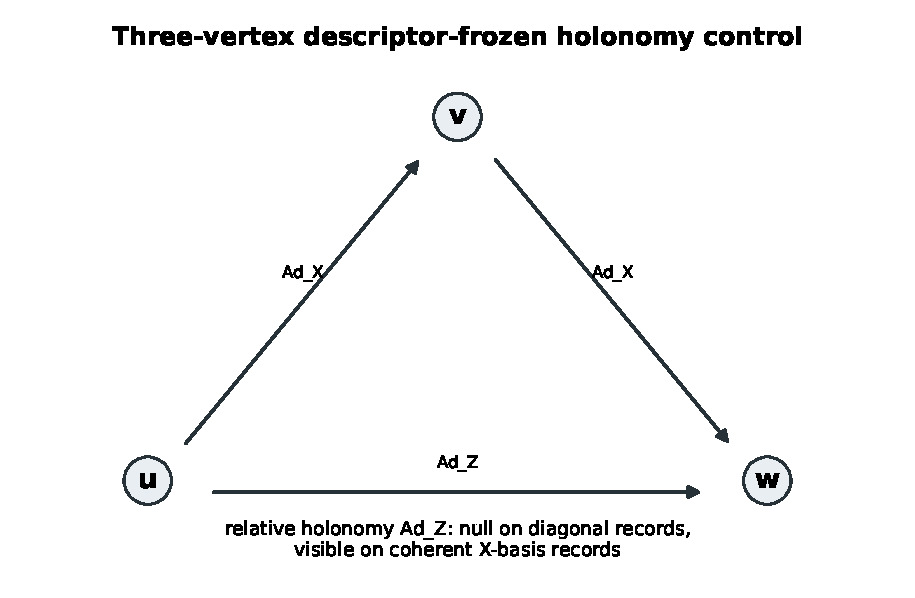
\includegraphics[width=0.78\linewidth]{figures/fig_holonomy_triangle.pdf}
 \caption{A three-vertex control.  The same relative automorphism is null on a
 diagonal record family but visible once a coherent \(X\)-basis witness is
 frozen into the endpoint descriptor.}
 \label{fig:holonomy-control}
\end{figure}

For a concrete control, take three fibers carrying \(M_2(\mathbb C)\), with
normalized trace, and edges
\begin{equation}
 \Pi_e=\Ad_X:u\to v,\qquad
 \Pi_f=\Ad_X:v\to w,\qquad
 \Pi_g=\Ad_Z:u\to w.
\end{equation}
For \(p=f\circ e\) and \(q=g\), \(\Pi_p=\id\) while
\(H_{p,q}=\Ad_Z\).  On diagonal densities and effects this holonomy is null.
If \(|+\rangle\langle+|\) and an \(X\)-basis effect are frozen into the
descriptor, \(\Ad_Z\) maps \(|+\rangle\) to \(|-\rangle\) and becomes visible.
The null decision therefore belongs to the predeclared operational claim, not
to an analyst's post-hoc choice.

\section{Irreversible CP relations}

A generic detector, decohering evolution or rank-reducing instrument is not a
complete edge.  If \(\mathcal C\) is CPTP, fidelity monotonicity gives
\begin{equation}
 F(\mathcal C(\rho),\mathcal C(\sigma))\geq F(\rho,\sigma),
 \qquad
 d_U^2(\mathcal C(\rho),\mathcal C(\sigma))
 \leq d_U^2(\rho,\sigma).
 \label{eq:cp-contraction}
\end{equation}
Exact finite A8b can therefore be lost.  It is restored on an occupied
domain if the map is exactly recoverable there.  The domain must be typed:

\begin{definition}[Recovery domains]
Let \(P\mathcal H\) be a code subspace.  We distinguish:
\begin{enumerate}[label=(R\arabic*)]
 \item a state family \(\mathfrak S\subseteq\mathsf D(P\mathcal H)\);
 \item a unital self-adjoint linear operator system
 \(\mathcal S_{\rm op}\subseteq\mathcal B(P\mathcal H)\);
 \item a correctable unital \(*\)-subalgebra
 \(\mathcal A_{\rm corr}\subseteq\mathcal B(P\mathcal H)\); and
 \item the full code algebra \(\mathcal B(P\mathcal H)\).
\end{enumerate}
State-family recovery means equality only on \(\mathfrak S\).  Operator-system
recovery means equality of the linear maps on \(\mathcal S_{\rm op}\).
Algebra recovery preserves all states and observables encoded by
\(\mathcal A_{\rm corr}\).  Full-code recovery is the special case
\(\mathcal A_{\rm corr}=\mathcal B(P\mathcal H)\).  None of these scopes may be
silently enlarged after the test.
\end{definition}

\begin{proposition}[Recovery sandwich]
Let \(\mathcal C\) and \(\mathcal R\) be CPTP maps satisfying
\begin{equation}
 (\mathcal R\circ\mathcal C)(\rho)=\rho
 \label{eq:exact-recovery}
\end{equation}
for every state in a frozen family \(\mathfrak S\).  Then for every pair
\(\rho,\sigma\in\mathfrak S\),
\begin{equation}
 F(\mathcal C(\rho),\mathcal C(\sigma))=F(\rho,\sigma),
 \qquad
 d_U^2(\mathcal C(\rho),\mathcal C(\sigma))=d_U^2(\rho,\sigma).
 \label{eq:recovery-isometry}
\end{equation}
\end{proposition}
\begin{proof}
Monotonicity under \(\mathcal C\) gives one inequality.  Applying monotonicity
under \(\mathcal R\) and using Eq.~\eqref{eq:exact-recovery} gives the reverse
inequality.  Equality of fidelity implies equality of the chord convention in
Eq.~\eqref{eq:quantum-separation}.
\end{proof}

This statement is closely related to quantum error-correction conditions
\cite{KnillLaflamme1997} and to the broader sufficiency/recovery viewpoint
\cite{Petz1986}, but only the explicit recovery identity is needed below.

\begin{proposition}[Explicit approximate-recovery chord bound]
Let \(\mathfrak S\) be a frozen state family and suppose
\begin{equation}
 \sup_{\rho\in\mathfrak S}
 \lVert(\mathcal R\mathcal C)(\rho)-\rho\rVert_1\leq\eta.
 \label{eq:state-family-recovery-error}
\end{equation}
This follows, in particular, from
\(\lVert\mathcal R\mathcal C-\id\rVert_\diamond\leq\eta\) on the full code
algebra.  For \(\rho,\sigma\in\mathfrak S\), define
\begin{equation}
 x_{\rm in}=d_U^2(\rho,\sigma),\qquad
 x_{\rm out}=d_U^2(\mathcal C\rho,\mathcal C\sigma).
\end{equation}
Then
\begin{equation}
 0\leq x_{\rm in}-x_{\rm out}
 \leq x_{\rm in}-
 \left[\max\{0,\sqrt{x_{\rm in}}-2\sqrt\eta\}\right]^2.
 \label{eq:approx-recovery-chord-bound}
\end{equation}
Equivalently,
\begin{equation}
 x_{\rm in}-x_{\rm out}
 \leq
 \begin{cases}
 x_{\rm in},&x_{\rm in}\leq4\eta,\\
 4\sqrt{\eta x_{\rm in}}-4\eta,&x_{\rm in}>4\eta.
 \end{cases}
 \label{eq:approx-recovery-piecewise}
\end{equation}
\end{proposition}
\begin{proof}
Write \(d(\rho,\sigma)=\sqrt{d_U^2(\rho,\sigma)}\), the Bures chord metric.
The Fuchs--van de Graaf inequality \cite{FuchsVandeGraaf1999} gives
\begin{equation}
 d\bigl(\rho,\mathcal R\mathcal C\rho\bigr)^2
 =2\bigl(1-\sqrt{F(\rho,\mathcal R\mathcal C\rho)}\bigr)
 \leq\lVert\rho-\mathcal R\mathcal C\rho\rVert_1\leq\eta,
\end{equation}
and likewise for \(\sigma\).  The triangle inequality and contractivity under
\(\mathcal R\) imply
\begin{equation}
 \sqrt{x_{\rm in}}
 \leq\sqrt{x_{\rm out}}+2\sqrt\eta.
\end{equation}
Contractivity under \(\mathcal C\) also gives
\(x_{\rm out}\leq x_{\rm in}\).  Solving these two inequalities for
\(x_{\rm out}\) yields Eqs.~\eqref{eq:approx-recovery-chord-bound} and
\eqref{eq:approx-recovery-piecewise}.
\end{proof}

The bound is useful only relative to the frozen domain.  It becomes weak when
\(x_{\rm in}\lesssim4\eta\), precisely where recovery error can hide the full
input separation.  It still concerns only the Uhlmann side; it does not make
the once-counted source action equal to either chord.

The estimate is exact in the limit \(\eta=0\) and becomes vacuous in the first
branch when \(x_{\rm in}\leq4\eta\).  It is a uniform worst-case consequence of
trace-norm recovery plus metric contractivity; no claim of universal
optimality is made for a specified channel, code, or state pair.  A smaller
state-dependent error may give a sharper bound, but it must be certified on
the same predeclared state family.  A diamond-norm certificate applies to the
full code including reference systems, whereas the state-family hypothesis in
Eq.~\eqref{eq:state-family-recovery-error} must not be silently promoted to
that stronger scope.

\section{A recovery-correctable CP toy model}

Let \(\mathcal H_L=\mathbb C^2\),
\(\mathcal H_P=(\mathbb C^2)^{\otimes3}\), and define the encoding isometry
\begin{equation}
 V|0\rangle=|000\rangle,\qquad V|1\rangle=|111\rangle.
 \label{eq:bitflip-encoding}
\end{equation}
Let \(X_i\) flip physical qubit \(i\), \(P_0=VV^\dagger\), and
\(P_i=X_iP_0X_i\).  These four syndrome subspaces are mutually orthogonal.
For \(0\leq p\leq1\), define
\begin{equation}
 \mathcal C_p(\rho)
 =(1-p)V\rho V^\dagger+{p\over3}\sum_{i=1}^3X_iV\rho V^\dagger X_i.
 \label{eq:bitflip-channel}
\end{equation}
This is CPTP and, for \(0<p<1\), is not a \(*\)-isomorphism from the logical
matrix algebra onto its noisy image.

Define a decoder by syndrome measurement and correction,
\begin{equation}
 \mathcal R_{\rm dec}(\sigma)=
 V^\dagger\!\left[P_0\sigma P_0+
 \sum_{i=1}^3X_iP_i\sigma P_iX_i\right]V
 +\Tr(P_{\rm fail}\sigma)|0\rangle\langle0|,
 \label{eq:bitflip-recovery}
\end{equation}
where \(P_{\rm fail}=I-P_0-\sum_iP_i\) makes the map trace preserving outside
the occupied range.

\begin{proposition}[Exact recovery-correctable non-isomorphic edge]
For every logical state \(\rho\),
\begin{equation}
 \mathcal R_{\rm dec}\circ\mathcal C_p(\rho)=\rho.
 \label{eq:toy-recovery-identity}
\end{equation}
Consequently Eq.~\eqref{eq:recovery-isometry} holds for all logical state
pairs and all \(p\in[0,1]\).
\end{proposition}
\begin{proof}
Each summand of Eq.~\eqref{eq:bitflip-channel} lies in one orthogonal syndrome
subspace.  The corresponding term in Eq.~\eqref{eq:bitflip-recovery} projects
onto that subspace, applies the matching correction, and decodes with \(V^\dagger\).
Every branch therefore returns its probability weight times \(\rho\); the
weights sum to one.  The recovery-sandwich proposition gives fidelity and
chord equality.
\end{proof}

The toy model recovers the full logical algebra
\(\mathcal B(\mathcal H_L)=M_2(\mathbb C)\), not merely a commuting state
family.  It proves that invertibility of the physical CP map is unnecessary
for exact finite metric transport on a certified code.  It does not show that
the body action assigns the same \(x_A\), nor that this code is a physical Tau
carrier.

\section{Why commuting records are insufficient}

Let \(\mathcal D\subset M_2(\mathbb C)\) be the diagonal algebra and compare
\begin{equation}
 \Pi_{\rm rev}=\id,
 \qquad
 \Pi_{\rm irr}(a)=P_0aP_0+P_1aP_1.
 \label{eq:dephasing-control}
\end{equation}
Both maps agree on every diagonal density and diagonal effect.  Yet
\(\Pi_{\rm irr}\) destroys off-diagonal coherence and has no CPTP inverse on
the full matrix algebra.

\begin{proposition}[Commuting-record reversibility no-go]
No protocol restricted to the commuting record algebra \(\mathcal D\) can
identify whether the occupied process is \(\Pi_{\rm rev}\) or
\(\Pi_{\rm irr}\).  Reversibility requires either a coherent witness outside
\(\mathcal D\) or a certified recovery test on a larger predeclared operator
system.
\end{proposition}
\begin{proof}
The two channels induce identical probabilities for every state and effect in
\(\mathcal D\).  Therefore every experiment confined to that algebra has the
same likelihood under both hypotheses.  An off-diagonal state/effect or a
recovery test separates them.
\end{proof}

\section{Why recovery is the relevant physical distinction}

The preceding results separate three statements that are often conflated.
First, an output may retain enough classical statistics to reproduce a chosen
endpoint table.  Second, a channel may preserve all pairwise state distances
on a declared family.  Third, a physical operation may admit a recovery on the
full operator system carrying that family.  Only the third statement certifies
that the apparently retained information was not silently converted into a
smaller commuting record.

This distinction matters for a morphological readout proposal because the
target identity \(x_A=x_Q\) concerns a finite state geometry, not merely one
probability distribution.  If the source-side action distinguishes coherent
directions that the observer process dephases, then a diagonal endpoint test
can report agreement while the claimed common geometry has already been lost.
The recovery domain therefore belongs to the physical claim:
\begin{equation}
 \text{action support}
 \supseteq \mathcal S_{\rm occ}
 \xrightarrow{\mathcal C}
 \mathcal C(\mathcal S_{\rm occ})
 \xrightarrow{\mathcal R}
 \mathcal S_{\rm occ}.
 \label{eq:recovery-claim-chain}
\end{equation}
If the last arrow is certified only on a state family, no conclusion about an
unmeasured coherent observable follows.  If it holds on a correctable algebra,
all encoded states and effects of that algebra are retained.  This is why the
paper keeps state-family, operator-system, algebra and full-code claims
separate rather than using ``information preserving'' as an untyped phrase.

\section{A quantitative nonrecoverable dephasing control}

Consider the qubit dephasing family
\begin{equation}
 \mathcal D_\lambda(\rho)
 ={1+\lambda\over2}\rho+{1-\lambda\over2}Z\rho Z,
 \qquad 0\leq\lambda\leq1.
 \label{eq:partial-dephasing}
\end{equation}
It fixes every diagonal state.  For the coherent pair
\begin{equation}
 \rho_+=|+\rangle\langle+|,
 \qquad
 \rho_-=|-\rangle\langle-|,
\end{equation}
the input states are orthogonal and hence
\begin{equation}
 x_{\rm in}=2.
\end{equation}
Their outputs have Bloch vectors \(\pm\lambda\hat x\).  The squared fidelity is
\begin{equation}
 F\bigl(\mathcal D_\lambda\rho_+,
        \mathcal D_\lambda\rho_-\bigr)=1-\lambda^2,
\end{equation}
so the output chord is
\begin{equation}
 x_{\rm out}(\lambda)=2\left(1-\sqrt{1-\lambda^2}\right).
 \label{eq:dephasing-chord}
\end{equation}
Thus \(x_{\rm out}(0)=0\), \(x_{\rm out}(1)=2\), and every
\(0\leq\lambda<1\) strictly contracts the coherent separation.  Meanwhile all
diagonal preparations and effects are exactly independent of \(\lambda\).

\begin{proposition}[Continuous hidden-contraction family]
No descriptor restricted to the diagonal algebra can estimate the coherent
chord loss in Eq.~\eqref{eq:dephasing-chord}.  A single predeclared
\(X\)-coherence witness identifies \(\lambda\) and therefore the lost finite
separation.
\end{proposition}
\begin{proof}
The restriction of \(\mathcal D_\lambda\) to the diagonal algebra is the
identity for every \(\lambda\), proving non-identifiability there.  On the
input \(\rho_+\), the expectation of \(X\) is
\(\Tr[X\mathcal D_\lambda(\rho_+)]=\lambda\).  Substitution into
Eq.~\eqref{eq:dephasing-chord} reconstructs the chord.
\end{proof}

This control is deliberately simpler than the three-qubit recovery example.
Together they bracket the decision: non-isomorphic and noisy need not mean
information-losing on a code, while perfect agreement on a classical record
need not mean preservation of the occupied quantum geometry.

\section{Carrier classes and admissible claims}

The theorem does not require one preferred hardware platform.  It requires a
carrier whose operational scope matches the claimed recovery scope.  Table
\ref{tab:carrier-classes} lists the minimum evidence for broad candidate
classes; none is asserted to be a Tau carrier.

\begin{table}[t]
\centering
\small
\begin{tabular}{p{0.22\linewidth}p{0.31\linewidth}p{0.36\linewidth}}
\toprule
Candidate class & Natural record support & Missing decisive certificate\\
\midrule
Superconducting or spin qubit
& Full two-level operator system with controllable coherent bases
& Independent source-action reconstruction and certified recovery/decoherence budget\\
Trapped ion or metastable atom
& Long-lived internal states with single-shot discrimination
& Same-carrier action curvature and held-record timing on a frozen protocol\\
Photon polarization/path
& High-quality tomography and explicit path holonomy
& Metastable one-record hold and separation of propagation loss from source geometry\\
Macroscopic pointer record
& Stable, redundant commuting outcomes
& Coherent witness or recovery on a larger operator system; diagonal stability alone is insufficient\\
\bottomrule
\end{tabular}
\caption{Candidate carrier classes and the evidence still needed before a
finite record packet can be promoted.  Familiar hardware supplies controls,
not the Tau-specific action--Uhlmann identity.}
\label{tab:carrier-classes}
\end{table}

The table also clarifies effect size.  A QOR timing test is meaningful only
after the finite geometry has been certified with uncertainty smaller than
the separation under test.  If \(\eta_{\rm rec}\) makes the upper bound in
Eq.~\eqref{eq:approx-recovery-piecewise} comparable to \(x_{\rm in}\), then
the carrier cannot distinguish a Tau-specific finite identity from ordinary
channel contraction, regardless of timing precision.

\section{Proof and falsification dependency}

The logical order of the paper is finite:
\begin{equation}
 \boxed{
 \begin{array}{c}
 \text{typed occupied support}\
 \Downarrow\\
 \text{complete edge or certified recovery}\
 \Downarrow\\
 \text{Uhlmann-chord preservation}\
 \Downarrow\quad\text{plus independent source action}\\
 x_A=x_Q\\
 \Downarrow\quad\text{plus held record and }\Delta H\\
 \text{QOR timing test}.
 \end{array}}
 \label{eq:dependency-spine}
\end{equation}
Failure at an earlier row cannot be repaired by a successful later timing
fit.  Conversely, failure of exact recovery need not reject every finite
readout model: it selects the approximate branch and requires the explicit
loss ledger of Eq.~\eqref{eq:approx-recovery-chord-bound}.  The decisive
falsification targets are therefore typed: failure of coherent/recovery
evidence rejects complete transport on the tested support; failure of
\(x_A=x_Q\) rejects the common-action identification; and a timing violation
rejects the occupied QOR completion only after both upstream certificates
have passed.

\subsection{Recovery-error budgets before timing}

For a target input chord \(x_*\), define the worst-case unresolved fractional
loss
\begin{equation}
 r_{\rm loss}(x_*,\eta)
 ={x_*-[\max\{0,\sqrt{x_*}-2\sqrt\eta\}]^2\over x_*}.
 \label{eq:fractional-loss-budget}
\end{equation}
The recovery certificate is informative at fractional tolerance \(r_0\) only
if \(r_{\rm loss}(x_*,\eta)\leq r_0\).  In the nonvacuous branch this is
equivalent to
\begin{equation}
 {4\sqrt{\eta x_*}-4\eta\over x_*}\leq r_0.
 \label{eq:recovery-budget-gate}
\end{equation}
This inequality must be checked before a timing run.  It prevents a small
observed body--state mismatch from being interpreted as new temporal physics
when ordinary channel uncertainty already permits the full discrepancy.

For illustration, Table~\ref{tab:recovery-budget} evaluates the certified
worst-case loss.  These are dimensionless mathematical controls, not predicted
experimental errors.

\begin{table}[t]
\centering
\small
\begin{tabular}{cccc}
\toprule
Target chord \(x_*\) & Recovery error \(\eta\) & Maximum chord loss & Fractional loss\\
\midrule
1.00 & \(10^{-2}\) & 0.36 & 36.0\%\\
1.00 & \(10^{-3}\) & 0.1225 & 12.25\%\\
0.25 & \(10^{-3}\) & 0.0592 & 23.68\%\\
0.25 & \(10^{-4}\) & 0.0196 & 7.84\%\\
\bottomrule
\end{tabular}
\caption{Worst-case losses from Eq.~\eqref{eq:approx-recovery-piecewise}.
Smaller target separations demand substantially stronger recovery
certificates.}
\label{tab:recovery-budget}
\end{table}

The scaling is important: at fixed \(\eta\), the relative uncertainty grows
as the target chord decreases.  A laboratory proposal should therefore not
begin with the smallest technically resolvable separation.  It should first
demonstrate the common-action identity at two or more separations for which
the recovery uncertainty is decisively subdominant, and only then test the
downstream timing relation.

\subsection{Frozen operational decision protocol}

A reproducible decision can be organized without assuming the Tau conclusion:
\begin{enumerate}[label=(P\arabic*)]
 \item Declare the state family or operator system, the source-action
 estimator and the allowed gauge before collecting endpoint data.
 \item Characterize \(\mathcal C\) and either certify a recovery map or freeze
 a coherent witness that detects departure from the commuting restriction.
 \item Choose at least two nonzero target separations satisfying
 Eq.~\eqref{eq:recovery-budget-gate} at the declared tolerance.
 \item Reconstruct \(x_A\) and \(x_Q\) independently and perform an equivalence
 test, not a failure-to-reject test, for the same-action identity.
 \item Only after P1--P4 pass, measure \(\Delta H\) and the held-record timing
 endpoint used in the QOR inequality.
 \item Run dephasing, drift, detector and nonlinear-response controls under the
 same analysis freeze.
\end{enumerate}

The corresponding verdicts are asymmetric.  Failure of P2 demotes the carrier
scope; failure of P4 rejects finite A8b on that scope; failure of P5 rejects
the occupied timing completion if the upstream certificates remain valid.
Passing all steps identifies one finite carrier packet within the tested model
class, not the complete Tau parent ontology.

\section{FOC-7 occupation certificate}

The preceding no-go upgrades the finite occupation certificate.  A candidate
carrier passes \emph{FOC-7} only if one predeclared protocol establishes:
\begin{enumerate}[label=(F\arabic*)]
 \item a metastable, held, single-shot record with a frozen discrimination
 error;
 \item independent source-side reconstruction of \(x_A\), without tomography
 or timing data;
 \item independent tomographic reconstruction of \(x_Q\);
 \item \(x_A=x_Q\) within predeclared equivalence margins at at least two
 nonzero separations;
 \item either a coherent off-diagonal witness distinguishing the complete
 operator system from its commuting restriction, or a certified recovery map
 satisfying \(\lVert\mathcal R\mathcal C-\id\rVert_\diamond\leq\eta_{\rm rec}\)
 on that system;
 \item downstream timing with independently measured energy spread; and
 \item controls for decoherence, drift, detector response and nonlinear finite
 corrections.
\end{enumerate}
Passing FOC-7 would identify the tested finite packet within its frozen model
class.  It would not by itself prove the entire parent ontology.  Failure at
F5 specifically prevents commuting data from being promoted into evidence for
a reversible complete edge.

\section{Projective loop invariants and the curvature boundary}

A conditional GNS/Gram packet sharpens the phase side of the present theory.
Write a nonzero overlap as $G_{ab}=r_{ab}U_{ab}$ with
$U_{ab}=e^{i\theta_{ab}}$.  Under local ray rephasing,
$|\chi_a\rangle\mapsto e^{i\alpha_a}|\chi_a\rangle$, one has
\begin{equation}
 U_{ab}\mapsto e^{-i\alpha_a}U_{ab}e^{i\alpha_b}.
\end{equation}
For a closed supported loop $\gamma=(a_1\ldots a_k a_1)$, the Bargmann
product and its phase,
\begin{equation}
 B_\gamma=\prod_{j=1}^{k}G_{a_j a_{j+1}},
 \qquad
 \Phi_\gamma=\arg B_\gamma,
 \label{eq:paperIII-bargmann}
\end{equation}
are gauge invariant.  If an overlap on the loop vanishes, the phase is not
defined and the support change must be treated separately.

For three normalized rays, Gram positivity gives the exact constraint
\begin{equation}
 1-r_{ab}^2-r_{bc}^2-r_{ca}^2
 +2r_{ab}r_{bc}r_{ca}\cos\Phi_{abc}\ge0.
 \label{eq:paperIII-gram-phase-bound}
\end{equation}
Thus magnitudes, loop phase and finite realizability are not independent.
Equation~\eqref{eq:paperIII-gram-phase-bound} also corrects a possible
overconstraint: consistency does not mean $\Phi_\gamma=0$.  Nonzero
projective holonomy is legitimate Hilbert geometry and must not be penalized
merely for being nontrivial.

The physical promotion remains open.  Equation~\eqref{eq:paperIII-bargmann}
does not by itself prove braid statistics, anyon support, a Parent
connection, spacetime curvature or Nature occupation.  Those conclusions
require, respectively, a source-owned configuration space and braid action,
a physical transport law on the same occupied carrier, and a derived map from
projective holonomy to a terminal observable.  The rigorous statement is
therefore
\begin{equation}
 \begin{aligned}
 \text{source-owned GNS probes}
 &\Longrightarrow \text{projective loop invariant},\\
 \text{projective loop invariant}
 &\not\Longrightarrow\text{physical curvature}.
 \end{aligned}
\end{equation}
This makes the overlap formulation useful to the paper while preserving its
existing source and occupation boundaries.

\section{What remains open}

\subsection{Later enriched-source status}

Inside the primary source-irredundant enriched completion, the traced
dagger-Frobenius two-leg record source, canonical represented trace and
primitive-extensive finite Trace--Gram law are now constructed conditionally
on the occupied complete ROOT path packet. Thus their internal construction is
no longer the principal gap. The cyclic generated-support criterion, together
with nonzero record unfolding and actual stable-record existence, now selects
complete source-packet occupation inside the declared source-irredundant MVP
carrier class. This does not yet supply the stronger transport hypotheses of
this paper: complete-edge invertibility, descriptor-complete holonomy descent,
or exact recovery on a stated operator system must still be certified.
Moreover, an inequivalent energy-sharing ownership completion has the same
current narrow source reduct, so transport or recovery success cannot identify
the unrestricted physical parent retroactively.

The operational physical-parent identity inherited from Paper IV narrows this
boundary without turning transport into a source selector. Complete-edge,
holonomy and recovery theorems act on the occupied seed-generated quotient
when the enriched one-source premise is adopted. A completely inert ambient
summand is physically null; a non-null transport difference at fixed complete
base--seed key is instead evidence for a second source or an incomplete
upstream signature. Recovery success alone proves neither alternative.

The later scalar-15/type-II branch does not change this transport boundary.
Its class-relative base--seed reconstruction closes which source packet owns
the selected branch, and its exact functional RG equation closes how that
packet is evaluated across scales.  Neither statement proves reversible
record transport, descriptor-complete holonomy descent or exact recovery.
In particular, the smooth RG cutoff must not be identified with the
observer-source finite-resolution map: the former is a removable calculation
scheme for an exact flow, whereas the latter defines operational readout
classes and must be physically sourced.

The internal mathematics now distinguishes three cases:
\begin{equation}
 \begin{array}{ccl}
 \text{complete reversible edge}&\Rightarrow&\text{exact finite Trace--Gram},\\
 \text{recovery-correctable CP edge}&\Rightarrow&\text{exact chord on the code},\\
 \text{generic irreversible CP edge}&\Rightarrow&\text{contraction or extra defect}.
 \end{array}
 \label{eq:three-case-fork}
\end{equation}
The decisive physical question is not settled by these implications:
\begin{quote}
Does the physical base--seed source create and occupy either the complete
dagger-Frobenius edge packet or a recovery-correctable non-isomorphic packet,
and does its once-counted action assign the same finite separation as the
observer amplitude geometry?
\end{quote}

The represented normalized trace and primitive extensivity are supplied
conditionally by the enriched traced source packet, rather than by local
Hessian positivity alone. Their unrestricted physical occupation remains an
input. Finite recovery completeness still says that the chord is a sufficient
statistic for action separation and remains separately falsifiable outside the
complete occupied path class.

Equation~\eqref{eq:approx-recovery-chord-bound} controls approximate recovery
on the frozen state family.  It is not an exact A8b theorem: the finite source
action remains independent, and experiment-specific promotion still requires
a declared code, error model and reconstruction uncertainty.

\subsection*{Inherited global-law obligation}

Complete and recovery-correctable record edges remain conditional on the
occupied parent completion.  Under the global source-fidelity/Hodge law,
positive-Schur extra topological sectors have zero effective source and remain
unoccupied.  This does not prove that Nature owns that law: an independent
component zero-jet can preserve every local transport datum while changing
the global minimum.  Physical promotion of an edge packet therefore requires
independent source derivation or empirical evidence for global-law ownership,
in addition to the transport and recovery tests proved here.

\subsection*{Relation to the unified selector}

PD-USS1 can use a source-owned reversible complete-edge transport as its
transport premise, but recovery-correctability or observed holonomy alone
does not supply the spectral grading identification or the actuality law.
Accordingly the updated $0/31$ cross-role data census is an acquisition result,
not evidence for physical complete-edge occupation. The recovery, dephasing
and braid-holonomy statements of this paper are unchanged.

\section{Conclusion}

The subsequent quantum-terminal closure also fixes the scope of the transport
results. For a logical source component separated from its inaccessible
complement by the occupied source hypergraph, a disjoint-source valuation
forces a block-diagonal parent Hessian and the complement carries no logical
input information; exact recovery then follows. A crossing occupied
hyperedge supplies the permitted interaction boundary, where entanglement,
leakage and local decoherence may occur while the joint state remains
represented. This does not assert unrestricted parent-law realization and
physical occupation of the valuation:
nonfaithful terminal descent can hide a parent cross term, so complete-edge
or recovery success on a restricted code cannot establish global parent
additivity.

Complete source-owned record edges provide a concise sufficient theorem for
finite action--Uhlmann identity, while path holonomy states exactly when that
identity can descend to endpoint-only data.  The operational descriptor makes
the null decision testable and prevents post-hoc removal of visible path
information.

Irreversibility does not end the route: the three-qubit construction proves
that a non-isomorphic CP map can preserve the Uhlmann chord on a certified
recoverable code.  But commuting record agreement is insufficient to decide
between this structure, a reversible edge, and dephasing.  FOC-7 therefore
requires coherent or recovery evidence in addition to action, tomography and
timing measurements.

The paper closes the internal finite alternatives, not their unrestricted
parent-law realization.  Physical source occupation, common-action ownership and a
laboratory carrier remain open empirical and source-theoretic problems.

This closes the series-level handoff without reversing it: architecture
precedes source identification, and source identification precedes transport.
An exact recovery theorem can preserve an occupied packet, but it cannot prove
that the physical base--seed parent law generates, realizes and occupies that
packet in the first place.
It also cannot prove that the Parent stored or successively rewrote the
recovered record.  Later conditioning may refine compatible histories while
the earlier marginal remains invariant; this is a downstream no-retro-
signalling consistency statement, not a record-transport proof of temporal
ontology.

\appendix
\section{Fidelity convention}

We use squared Uhlmann fidelity
\begin{equation}
 F(\rho,\sigma)=\left[\Tr\sqrt{\sqrt\rho\,\sigma\sqrt\rho}\right]^2.
\end{equation}
The minimum Hilbert--Schmidt purification chord is
\begin{equation}
 \min_U\lVert W_\rho-W_\sigma U\rVert_{\HS}^2
 =2(1-\sqrt F),
\end{equation}
following Uhlmann's purification geometry \cite{Uhlmann1976}.  This is not the
squared Bures distance convention used in every part of the literature; all
equalities in this paper use the displayed definition.

\bibliographystyle{unsrt}
\bibliography{refs}

\end{document}
